\documentclass[a4paper,12pt,oneside,openany]{memoir}
\input{../../preamble.tex}
\graphicspath{{images/}{../practice8/images/}}

% Данные для титульника
\newcommand{\practiceNumber}{8}
\newcommand{\practiceTitle}{Реалзиация символьной синхронизации. Применение к сэмплам с
AdalmPluto. Разработка графического интерфейса (GUI) для работы с SDR.
Окна настроек SDR, вывод результатов обработки сэмплов и т.д.}
\newcommand{\studentName}{К.А Любимов}
\newcommand{\studentGroup}{ИА-331}
\newcommand{\practiceYear}{2026}

\begin{document}

% Титульник практики
\input{title_practice8.tex}

% Содержание практики
\chapter[Реалзиация символьной синхронизации. Применение к сэмплам с
AdalmPluto. Разработка графического интерфейса (GUI) для работы с SDR.
Окна настроек SDR, вывод результатов обработки сэмплов и т.д.]{Реалзиация символьной синхронизации. Применение к сэмплам с
AdalmPluto. Разработка графического интерфейса (GUI) для работы с SDR.
Окна настроек SDR, вывод результатов обработки сэмплов и т.д.}

\begin{leftbar}
    \href{https://github.com/someotb/sdr}{Ссылка на GitHub}
\end{leftbar}

\section*{Цель практики:}

Написать алгоритм который будет выполнять символьную синхронизацию приемника и передатчика. Написать графический интерфейс, который будет
выводить данные в реальном времени с помощью Dear ImGUI, ImPlot.

\section*{Краткие теоретические сведения}

Символьная синхронизация это алгоритм, который находит начало полезного сигнала. Я сделал его с помощью PSS.
А именно с помощью последовательности Zadoff-Chu. Графический интерфей был написан с помощью библиотеки Dear ImGui, а сопутсвующие графики
с помощью дополнения ImPlot.

\vspace{10pt}

\textbf{Символьная синхронизация по Zadoff-Chu}\newline
Последовательности Задова-Чу (Zadoff-Chu) — это CAZAC-последовательности (constant amplitude zero autocorrelation): комплексные последовательности с постоянной амплитудой и нулевой периодической автокорреляцией при любом ненулевом сдвиге. В LTE/5G применяются для синхронизации (PSS — Primary Synchronization Signal) и для преамбул случайного доступа (PRACH), потому что приёмник может по пику корреляции точно определить временной сдвиг сигнала, а разные корневые индексы последовательности дают взаимно почти ортогональные (низкая кросс-корреляция) сигналы — это позволяет разным базовым станциям/пользователям использовать разные ZC-последовательности без сильной взаимной интерференции.

Механика: последовательность генерируется как $x_u(n) = e^{-j\pi u n(n+1)/N}$ (для нечётного N), где $u$ — корневой индекс, взаимно простой с N. Идеальная нулевая автокорреляция сохраняется только для циклического сдвига внутри одного периода — на практике приёмник использует именно это свойство, ища по корреляции с локальной копией пик, соответствующий временной задержке до передатчика.

\textbf{Dear ImGui, ImPlot}\newline
Dear ImGui — библиотека для GUI в режиме immediate mode: интерфейс не хранится как дерево объектов, а переописывается каждый кадр вызовами функций, которые сразу и рисуют виджет, и возвращают результат взаимодействия. Она не занимается рендерингом и вводом сама — это делает backend (DirectX/OpenGL/Vulkan) и ОС.

ImPlot — надстройка над ImGui той же логики, но для графиков: линии, гистограммы, heatmaps описываются между `BeginPlot`/`EndPlot`, данные берутся по указателю без копирования, что удобно для данных, меняющихся каждый кадр.


\section*{Выполнение}

Напишем функцию, которая будет строить последовательность Zadoff-Chu:

\begin{lstlisting}[language=C++, caption=Функция построения последовательности Zadoff-Chu]
void build_pss_zadoff_chu(FFT_Context &context, sharedData &sd)
{
    int N_zc = sd.subcarrier - 1;
    int cf = N_zc % 2;
    int q = 1;

    for (int i = 0; i < context.N; ++i)
    {
        context.in[i][0] = 0.0f;
        context.in[i][1] = 0.0f;
    }

    for (int n = 0; n < N_zc; ++n)
    {
        float phase = -(M_PIf * (float)sd.zadoff_chu_u * (float)n * (float)(n + cf + 2 * q)) / (float)N_zc;
        float sin, cos;
        sin = sinf(phase);
        cos = cosf(phase);
        context.in[n][0] = cos;
        context.in[n][1] = sin;
    }

    context.ifft();
}
\end{lstlisting}

Она строит последовательность, записывает сэмплы в специальный массив ищ библиотеки fftw3, которая делает быстро преобразование Фурье. И сразу в этой
функции делается обратное преобразование Фурье, за это отвечается строка: `context.ifft();`

\vspace{20pt}

\begin{lstlisting}[language=C++, caption=Функци корреляции Zadoff-Chu]
int zadoff_sync(const float *signal_re, const float *signal_im, size_t signal_len, const float *zc_re,
                const float *zc_im, size_t zc_len, float *out_corr)
{
    float max_norm = -1.f;
    int best_idx = 0;

    for (size_t n = 0; n < signal_len - zc_len; ++n)
    {
        float sum_re = 0.0f;
        float sum_im = 0.0f;

        for (size_t k = 0; k < zc_len; ++k)
        {
            sum_re += signal_re[n + k] * zc_re[k] + signal_im[n + k] * zc_im[k];
            sum_im += signal_im[n + k] * zc_re[k] - signal_re[n + k] * zc_im[k];
        }

        float cur_norm = sum_re * sum_re + sum_im * sum_im;

        if (out_corr)
            out_corr[n] = cur_norm;

        if (cur_norm > max_norm)
        {
            max_norm = cur_norm;
            best_idx = (int)n;
        }
    }
    return best_idx;
}
\end{lstlisting}

На вход функция принимает сырые const float указатели, это делается для ускорения выполнения алгоритма, потому что корреляция довольно трудоемкий процесс,
а в моей системе важна скорость. Иначе, мой код просто не будет успевать обрабатывать буферы сэмплов. На выходе мы получаем индекс в массиве, который имеет наивысший пик корреляции
с известной последовтельностью Zadoff-Chu.

\begin{figure}[H]
    \centering
    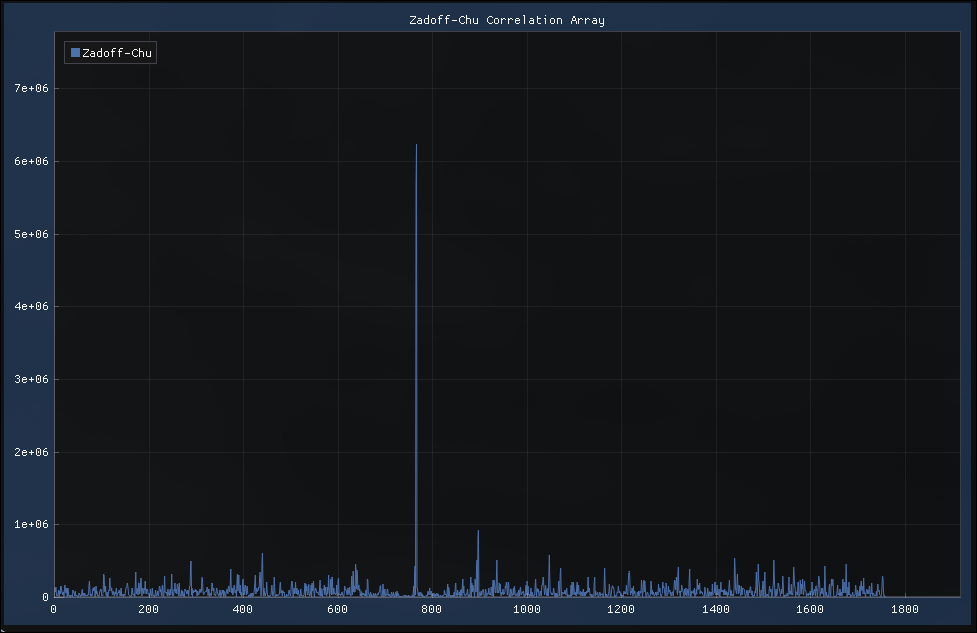
\includegraphics[width=0.7\textwidth]{zadoff-chu_peak.jpg}
    \caption{График пика корреляции последовательности Zadoff-Chu на всем буфере}
\end{figure}

\vspace{20pt}

Графический интерфейс написан на Dear ImGui, в качестве backend идет OpenGL3, в качестве библиотки для обработки действий пользователя идет
GLWF3. Также была выбрана экспериментальная ветка с функцией docking. В этой ветке у внутренних окон есть возможность примагничиваться к крайм экрана и друг к другу.
Это позволяет более гибко настраивать рабочую область.

В коде сперва идет инициализация окна и всего прочего, а затем уже создаются окна, подокна и т.д.

\begin{lstlisting}[language=C++, caption=Инициализация окон]
glfwWindowHint(GLFW_CONTEXT_VERSION_MAJOR, 3);
glfwWindowHint(GLFW_CONTEXT_VERSION_MINOR, 3);
glfwWindowHint(GLFW_OPENGL_PROFILE, GLFW_OPENGL_CORE_PROFILE);

#ifdef __APPLE__
    glfwWindowHint(GLFW_OPENGL_FORWARD_COMPAT, GL_TRUE);
#endif

GLFWwindow* window = glfwCreateWindow(1280, 720, "SDR", nullptr, nullptr);
if (!window) return;
glfwMakeContextCurrent(window);
glfwSwapInterval(1);

IMGUI_CHECKVERSION();
ImGui::CreateContext();
ImPlot::CreateContext();
ImGui::StyleColorsDark();

static std::string ini_path = "../config/imgui.ini";
ImGuiIO &io = ImGui::GetIO();
io.IniFilename = ini_path.c_str();

ImGui::GetIO().ConfigFlags |= ImGuiConfigFlags_DockingEnable;
ImGui::GetIO().ConfigFlags |= ImGuiConfigFlags_ViewportsEnable;

ImGui_ImplGlfw_InitForOpenGL(window, true);
ImGui_ImplOpenGL3_Init("#version 330");

while (!glfwWindowShouldClose(window))
{
    glfwPollEvents();
    ImGui_ImplOpenGL3_NewFrame();
    ImGui_ImplGlfw_NewFrame();
    ImGui::NewFrame();
    ImGui::DockSpaceOverViewport(0, ImGui::GetMainViewport());

    // Start GUI
\end{lstlisting}

Вот так выглядит подготовка к созданию окон и контекстов.

\begin{lstlisting}[language=C++, caption=Пример построения графика]
if (ImGui::Begin("Scatter Raw"))
{
    if (ImPlot::BeginPlot("Raw Samples", ImVec2(ImGui::GetContentRegionAvail())))
    {
        if (!local_raw.empty())
        {
            ImPlotSpec spec;
            spec.Stride = sizeof(std::complex<float>);
            ImPlot::PlotScatter("I/Q", raw_data, raw_data + 1, local_raw.size(), spec);
            ImPlot::EndPlot();
        }
        else
        {
            ImPlot::Annotation(0.5, 0.5, ImVec4(1, 0, 0, 1), ImVec2(0, 0), true, "No Data");
            ImPlot::EndPlot();
        }
    }
}
ImGui::End();
\end{lstlisting}

Для создания окон используется ImGui::Begin(); ... ImGui::End();

\begin{figure}[H]
    \centering
    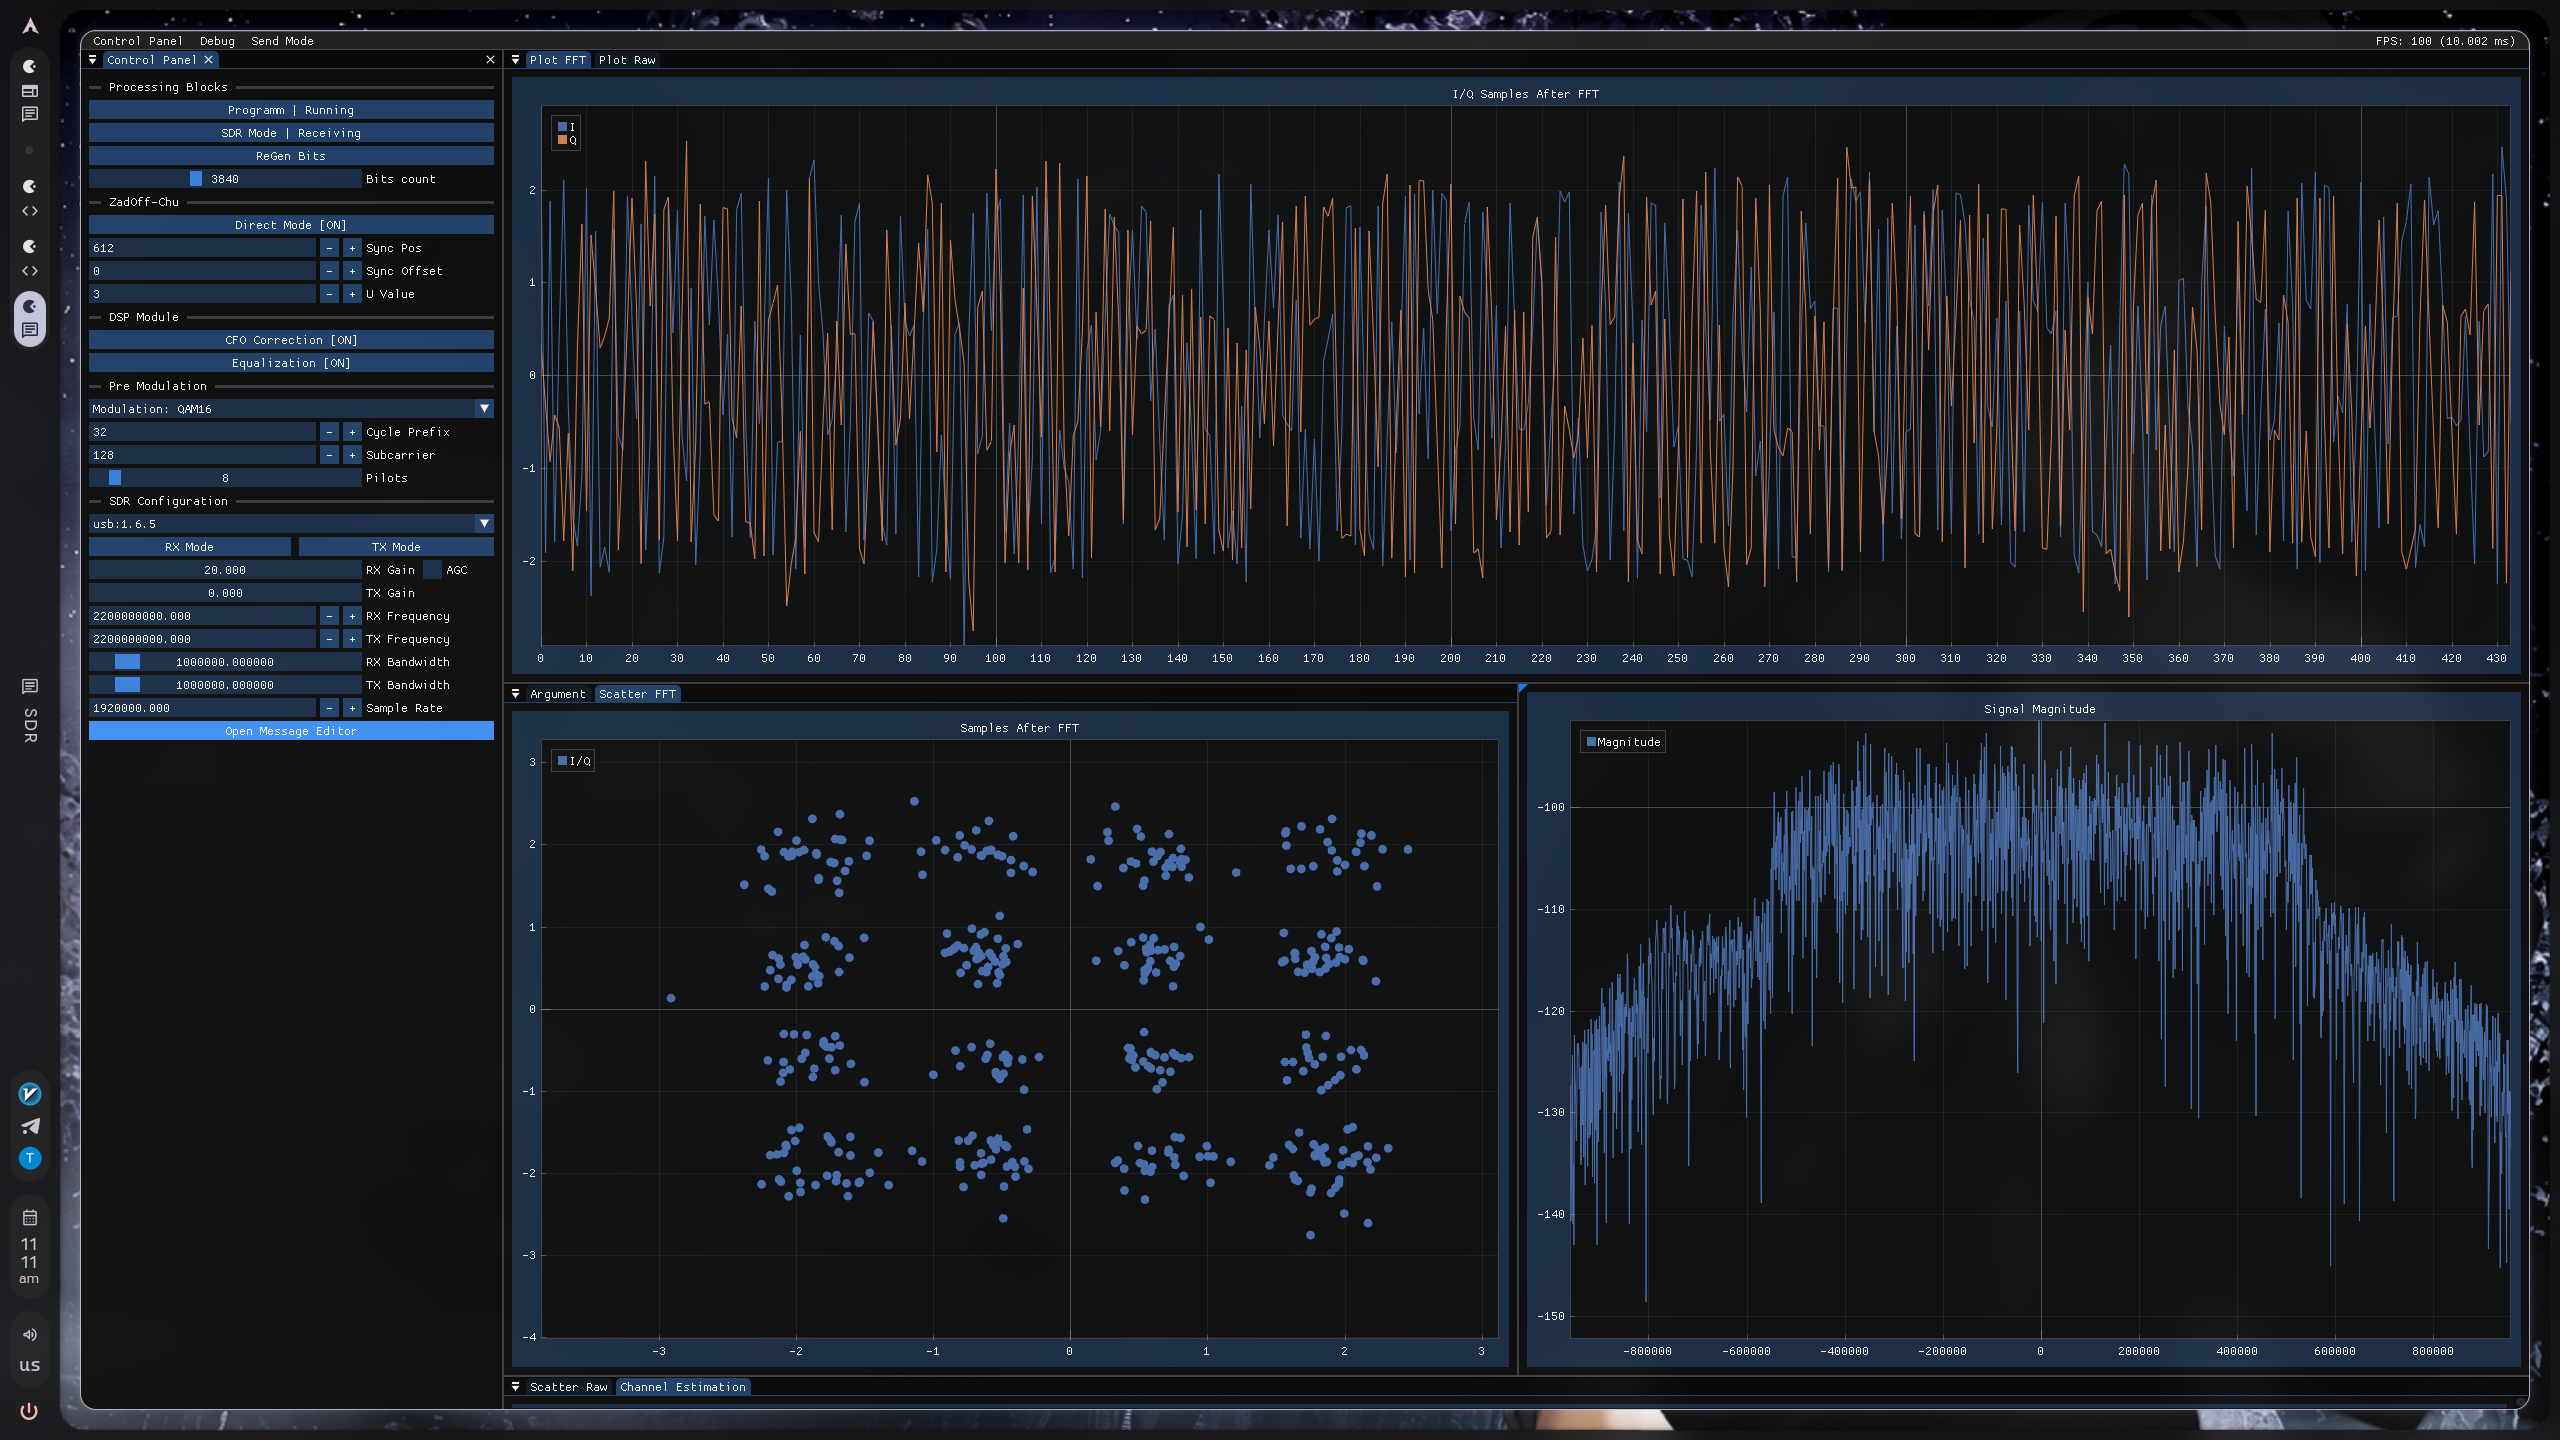
\includegraphics[width=1.0\textwidth]{gui.jpg}
    \caption{Как выгядит GUI}
\end{figure}

\section*{Вывод}
Была написан алогоритм символьной синхронизации, который работает по последовательности Zadoff-Chu. Написан графический интерфейс при помощи библиотки Dear ImGui, на базе OpenGL3 и GLWF3.


\end{document}
